\documentclass[a4paper]{article}
\usepackage[utf8]{inputenc}
\usepackage[T1]{fontenc}
\usepackage[french]{babel}
\usepackage{graphicx}
\usepackage{algorithmeUTF8}
\usepackage[left=3cm,right=3cm,top=3cm,bottom=3cm]{geometry}
\usepackage{minted}
\newcommand{\noun}[1]{\textsc{#1}}

\title{Projet Ruzzle}
\author{Nina \noun{Lardiere}, Yves \noun{Le Guennec}, Simon \noun{Lebeaud}, Tanguy \noun{Leclerc}}
\date{Octobre 2018 - Janvier 2019}

\begin{document}
	\maketitle
	\tableofcontents
	\newpage
	\section{Introduction}
	Dans le cadre du projet d'algorithmique enseigné par M.Delestre en 3ème année, nous avions comme sujet à traité la résolution de grille du jeu Ruzzle. Ce jeu consiste à faire le plus de mot possible avec une grille 4\times4 de lettres différentes. Chaque lettre ayant un score, et possiblement un bonus. La résolution d'une telle grille ce fait en trouvant tout les mots contenu dans cette grille.
	Tout les mots possible nous ont d'abord été transmit sous la forme d'un fichier texte. Le but de ce projet était donc de mettre en oeuvre un programme permettant la résolution de telles grilles et de ranger tout les mots obtenu celon le score quu'ils produisent. Ce projet est d'abord la première application de nos connaissances acquisent en cours d'algorithmique durant le semestre 3.1.

	\section{Analyse}
		\subsection{Les TAD}
			\begin{tad}
  \tadNom{Case}
  \tadDependances{A..Z,\naturelNonNul,Bonus,1..4}
  \begin{tadOperations}{obtenirNbPoints}%nom de l'opération le plus long
    \tadOperation{creerCase}{}{\tadUnParam{Case}}
    \tadOperation{fixerLettre}{\tadDeuxParams{Case}{A..Z}}{\tadUnParam{Case}}
    \tadOperation{fixerNbPoints}{\tadDeuxParams{Case}{\naturelNonNul}}{\tadUnParam{Case}}
    \tadOperation{fixerBonus}{\tadDeuxParams{Case}{Bonus}}{\tadUnParam{Case}}
    \tadOperation{obtenirLettre}{\tadUnParam{Case}}{\tadUnParam{A..Z}}
    \tadOperation{obtenirNbPoints}{\tadUnParam{Case}}{\tadUnParam{\naturelNonNul}}
    \tadOperation{obtenirBonus}{\tadUnParam{Case}}{\tadUnParam{Bonus}}
    \tadOperation{obtenirPosX}{\tadUnParam{Case}}{\tadUnParam{1..4}}
    \tadOperation{obtenirPosY}{\tadUnParam{Case}}{\tadUnParam{1..4}}
    \tadOperation{fixerPosition}{\tadTroisParams{Case}{1..4}{1..4}}{\tadUnParam{Case}}
  \end{tadOperations}
  \begin{tadAxiomes}
    \tadAxiome{obtenirLettre(creerCase())='A'}
    \tadAxiome{obtenirNbPoints(creerCase())=1}
    \tadAxiome{obtenirBonus(creerCase())="\textvisiblespace\textvisiblespace"}
    \tadAxiome{obtenirLettre(fixerLettre(uneCase,uneLettre))=uneLettre}
    \tadAxiome{obtenirBonus(fixerBonus(uneCase,leBonus))=leBonus}
    \tadAxiome{obtenirNbPoints(fixerNbPoints(uneCase,nbPoints))=nbPoints}
    \tadAxiome{obtenirPosX(fixerPosition(uneCase,x,y))=x}
    \tadAxiome{obtenirPosY(fixerPosition(uneCase,x,y))=y}
  \end{tadAxiomes}
\end{tad}
\medskip

\begin{tad}
  \tadNom{Grille}
  \tadDependances{Case,\booleen,1..4}
  \begin{tadOperations}{DebutUtilisation}%nom de l'opération le plus long
      \tadOperation{creerGrille}{}{\tadUnParam{Grille}}
      \tadOperation{obtenirCase}{\tadTroisParams{Grille}{1..4}{1..4}}{\tadUnParam{Case}}
      \tadOperation{fixerCase}{\tadQuatreParams{Grille}{Case}{1..4}{1..4}}{\tadUnParam{Grille}}
      \tadOperation{estUtilisee}{\tadTroisParams{Grille}{1..4}{1..4}}{\tadUnParam{\booleen}}
      \tadOperation{debutUtilisation}{\tadTroisParams{Grille}{1..4}{1..4}}{\tadUnParam{Grille}}
      \tadOperation{finUtilisation}{\tadTroisParams{Grille}{1..4}{1..4}}{\tadUnParam{Grille}}
  \end{tadOperations}
  \begin{tadAxiomes}
    \tadAxiome{obtenirCase(creerGrille,x,y)=creerCase()}
    \tadAxiome{obtenirCase(fixerCase(c,x,y))=c}
    \tadAxiome{estUtilisee(debutUtilisation(g,x,y))=VRAI}
    \tadAxiome{estUtilisee(finUtilisation(g,x,y))=FAUX}
  \end{tadAxiomes}
\end{tad}
\medskip

\begin{tad}
  \tadNom{Mot}
  \tadDependances{Dictionnaire,\chaine,\naturelNonNul,\caractere}
  \begin{tadOperations}{ajouterLettre}%nom de l'opération le plus long
    \tadOperationAvecPreconditions{chaineEnMot}{\tadDeuxParams{Dictionnaire}{\chaine}}{\tadUnParam{Mot}}
    \tadOperation{motEnChaine}{\tadUnParam{Mot}}{\tadUnParam{\chaine}}
    \tadOperation{longueur}{\tadUnParam{Mot}}{\tadUnParam{\naturelNonNul}}
    \tadOperationAvecPreconditions{ajouterLettre}{\tadTroisParams{Dictionnaire}{Mot}{\caractere}}{\tadUnParam{Mot}}
    \tadOperationAvecPreconditions{retirerLettre}{\tadUnParam{Mot}}{\tadUnParam{Mot}}
  \end{tadOperations}
  \begin{tadPreconditions}{retirerLettre}
    \tadPrecondition{chaineEnMot}{estUnPrefixe(dico,chaine) ET longueur(chaine)$\geq$1}
    \tadPrecondition{ajouterLettre}{estUnPrefixe(dico,motEnChaine(unMot)+lettre)}
    \tadPrecondition{retirerLettre}{longueur(unMot) $\geq$ 2}
   \end{tadPreconditions}
   \begin{tadAxiomes}
     \tadAxiome{motEnChaine(chaineEnMot(dico,uneChaine))=uneChaine}
     \tadAxiome{motEnChaine(ajouterLettre(dico,unMot,lettre))=motEnChaine(unMot)+lettre}
     \tadAxiome{longueur(ajouterLettre(dico,unMot,lettre))=longueur(unMot)+1}
     \tadAxiome{longueur(retirerLettre(unMot))=longueur(unMot)-1}
   \end{tadAxiomes}
\end{tad}
\medskip

\begin{tad}
  \tadNom{Dictionnaire}
  \tadDependances{Mot,\chaine,Fichier,\booleen}
  \begin{tadOperations}{obtenirLettresSuivantes}%nom de l'opération le plus long
    \tadOperation{creerDictionnaire}{\tadUnParam{Ensemble<\chaine>}}{\tadUnParam{Dictionnaire}}
    \tadOperation{ajouterMot}{\tadDeuxParams{Dictionnaire}{\chaine}}{\tadUnParam{Dictionnaire}}
    % pas nécessaire pour le Ruzzle, tous les mots étant contenus dans le fichier utilisé par creerDictionnaire
    \tadOperationAvecPreconditions{supprimerMot}{\tadDeuxParams{Dictionnaire}{Mot}}{\tadUnParam{Dictionnaire}}
   % pas nécessaire pour le Ruzzle
    \tadOperation{estUnPrefixe}{\tadDeuxParams{Dictionnaire}{\chaine}}{\tadUnParam{\booleen}}
    \tadOperation{estUnMot}{\tadDeuxParams{Dictionnaire}{Mot}}{\tadUnParam{\booleen}}
    \tadOperation{obtenirLettresSuivantes}{\tadDeuxParams{Dictionnaire}{Mot}}{\tadUnParam{Ensemble<A..Z>}}
    \tadOperation{sauvegarder}{\tadUnParam{Dictionnaire}}{\tadUnParam{Fichier}}
    \tadOperation{charger}{\tadUnParam{Fichier}}{\tadDeuxParams{Dictionnaire}{\booleen}}
  \end{tadOperations}
  \begin{tadPreconditions}{retirerLettre}
    \tadPrecondition{supprimerMot}{estUnMot(motASupprimer)}
   \end{tadPreconditions}
  \begin{tadSemantiques}{obtenirLettresSuivantes}
    \tadSemantique{creerDictionnaire}{création d'un dictionnaire à partir d'une suite de mots}
    \tadSemantique{ajouterMot}{ajout d'un mot dans le dictionnaire}
    \tadSemantique{supprimerMot}{suppression d'un mot du dictionnaire}
    \tadSemantique{estUnPrefixe}{indique si la suite de caractères est le début d'un mot du dictionnaire}
    \tadSemantique{estUnMot}{indique si le préfixe est un mot complet}
    \tadSemantique{obtenirLettresSuivantes}{indique, pour un préfixe donné, toutes les lettres qui peuvent suivre le préfixe pour former un nouveau préfixe}
    \tadSemantique{sauvegarder}{sauvegarde le dictionnaire dans un fichier}
    \tadSemantique{charger}{charge le dictionnaire à partir d'un fichier préalablement généré par l'opération sauvegarder}
  \end{tadSemantiques}
\end{tad}
\medskip

\begin{tad}
  \tadNom{CasesContigues}
  \tadDependances{Case,\naturel,\chaine}
  \begin{tadOperations}{CasesContiguesEnChaine}
    \tadOperation{creerCasesContigues}{}{\tadUnParam{CasesContigues}}
    \tadOperation{ajouterCase}{\tadDeuxParams{CasesContigues}{Case}}{\tadUnParam{CasesContigues}}
    \tadOperationAvecPreconditions{supprimerCase}{\tadUnParam{CasesContigues}}{\tadUnParam{CasesContigues}}
    \tadOperation{nbCasesContigues}{\tadUnParam{CasesContigues}}{\tadUnParam{\naturel}}
    \tadOperation{casesContiguesEnChaine}{\tadUnParam{CasesContigues}}{\tadUnParam{\chaine}}
  \end{tadOperations}
  \begin{tadPreconditions}{supprimerCase}
     \tadPrecondition{supprimerCase}{nbCasesContigues(suiteCases) $>$ 0}
  \end{tadPreconditions}
  \begin{tadAxiomes}
    \tadAxiome{supprimerCase(ajouterCase(suiteCases,uneCase))=uneCase}
    \tadAxiome{nbCasesContigues(creerCasesContigues())=0}
  \end{tadAxiomes}
\end{tad}


		\subsection{Analyse descendante}
			voir Figure \ref{fig:AD}
			\begin{figure}
				\centering 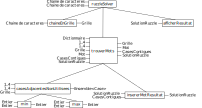
\includegraphics[width=1\textwidth]{./analyseDescendante/analyseDescendante}
				\caption{\label{fig:AD}Analyse descendante}
			\end{figure}

	\newpage
	\section{Conception préliminaire}
		\subsection{Signatures des fonctions et procédures des TAD}
			\paragraph{Case}
\begin{algorithme}
  \signaturefonction
  {creerCase}{}{Case}

  \signatureprocedure
  {fixerLettre}{\paramEntreeSortie{c : Case}; \paramEntree{uneLettre : A..Z}}

  \signatureprocedure
  {fixerNbPoints}{\paramEntreeSortie{c : Case}; \paramEntree{nbPoints : \naturelNonNul}}

  \signatureprocedure
  {fixerBonus}{\paramEntreeSortie{c : Case}; \paramEntree{bonus : Bonus}}

  \signaturefonction
  {obtenirLettre}{c : Case}{A..Z}

  \signaturefonction
  {obtenirNbPoints}{c : Case}{\naturelNonNul}

  \signaturefonction
  {obtenirBonus}{c : Case}{Bonus}

  \signatureFonction{obtenirPosX}{c : Case}{1..4}
  \signatureFonction{obtenirPosY}{c : Case}{1..4}
  \signatureProcedure{fixerPosition}{\paramEntreeSortie{c : Case} \paramEntree{posX, posY : 1..4}}
\end{algorithme}

\paragraph{Grille}
\begin{algorithme}
  \signaturefonction
  {creerGrille}{}{Grille}

  \signaturefonction
  {obtenirCase}{g : Grille ; coordX, coordY : 1..4 }{Case}

  \signatureprocedure
  {fixerCase}{\paramEntreeSortie{g : Grille}; \paramEntree{c :Case ; coordX, coordY : 1..4}}

  \signaturefonction
  {estUtilisee}{g : Grille ; coordX, coordY : 1..4}{\booleen}

  \signatureprocedure
  {debutUtilisation}{\paramEntreeSortie{g : Grille}; \paramEntree{xUtilisee, yUtilisee : 1..4}}

  \signatureprocedure
  {finUtilisation}{\paramEntreeSortie{g : Grille}; \paramEntree{xUtilisee, yUtilisee : 1..4}}

\end{algorithme}

			\paragraph{CasesContigues}
\begin{algorithme}
	\signaturefonction{creerCasesContigues}{}{CasesContigues}
	\signatureprocedure{ajouterCase}{\paramEntreeSortie{suiteCases : CasesContigues} \paramSortie{uneCase : Case}}
	\signatureProcedureAvecPreconditions {supprimerCase}{\paramEntreeSortie{suiteCases : CasesContigues}}{nbCasesContigues(suiteCases) $>$ 0}
	\signaturefonction{nbCasesContigues}{suiteCase : CasesContigues}{\naturel}
	\signaturefonction{casesContiguesEnChaine}{suiteCases : CasesContigues}{\chaine}
\end{algorithme}

			\paragraph{Mot}
\begin{algorithme}
  \signaturefonctionAvecPrecondition
  {chaineEnMot}{dico : Dictionnaire ; ch : \chaine}{mot : Mot}{estUnPrefixe(dico,chaine) ET longueur(chaine)$\geq$1}

  \signaturefonction
  {motEnChaine}{mot : Mot}{ch : \chaine}
  
  \signaturefonction
  {longueur}{mot : Mot}{n : \naturelNonNul}
  
  \signatureProcedureAvecPreconditions 
  {ajouterLettre}{\paramEntreeSortie{mot : Mot} \paramEntree{car : \caractere; dico : Dictionnaire}}{estUnPrefixe(dico,motEnChaine(unMot)+lettre)}
  
  \signatureProcedureAvecPreconditions 
  {retirerLettre}{\paramEntreeSortie{mot : Mot}}{estUnPrefixe(dico,motEnChaine(unMot)+lettre)}

\end{algorithme}

			\paragraph{Dictionnaire}
\begin{algorithme}

  \signaturefonction
  {creerDictionnaire}{lesMots : Ensemble<\chaine>}{Dictionnaire}

  \signatureProcedure
  {ajouterMot}{\paramEntreeSortie{dico : Dictionnaire} \paramEntree{leMot : \chaine}}
  % pas nécessaire pour le Ruzzle, tous les mots étant contenus dans le fichier utilisé par creerDictionnaire

  \signatureProcedureAvecPreconditions
  {supprimerMot}{\paramEntreeSortie{dico : Dictionnaire} \paramEntree{motASupprimer : Mot}}{estUnMot(motASupprimer)}

  % pas nécessaire pour le Ruzzle
  \signaturefonction
  {estUnPrefixe}{dico : Dictionnaire ; chaine : \chaine}{\booleen}

  \signaturefonction
  {estUnMot}{dico : Dictionnaire ; prefixe : Mot}{\booleen}

  \signaturefonction
  {obtenirLettresSuivantes}{dico : Dictionnaire ; prefixe : Mot}{Ensemble<A..Z>}

  \signatureProcedure
  {sauvegarder}{\paramEntree{dico : Dictionnaire}}

  \signatureProcedure
  {charger}{\paramEntree{fichier : Fichier} \paramSortie{dico : Dictionnaire ; erreur : \booleen}}

\end{algorithme}


		\subsection{Signatures des fonctions et procédures de l'analyse descendante}
			\begin{algorithme}
  \signatureprocedure
    {ruzzleSolver}
    {
      \paramEntree{grilleRuzzle, nomFichierDico: \chaine}
    }

  \signaturefonction
    {chaineEnGrille}
    {\chaine}
    {Grille}

  \signatureprocedure
    {trouverMots}
    {
      \paramEntree{posX, posY: 1..4 ; dico: Dictionnaire}
      \paramEntreeSortie{g: Grille; prefixe: Mot; cheminRuzzle : CasesContigues, resultat: SolutionRuzzle}
    }

  \signatureprocedure
    {afficherResultat}
    {
      \paramEntree{resultat: SolutionRuzzle}
    }

  \signaturefonction
    {casesAdjacentesNonUtilisees}
    {posX, posY : 1..4 ; g : Grille}
    {Ensemble<Case>}

  \signaturefonction
    {min}
    {a,b : \entier}
    {\entier}

  \signaturefonction
    {max}
    {a,b : \entier}
    {\entier}

  \signatureprocedure
    {insererMotResultat}
    {
      \paramEntree{cheminRuzzle : CasesContigues}
      \paramEntreeSortie{resultat: SolutionRuzzle}
    }

\end{algorithme}


	\newpage
	\section{Conception détaillée}
		\begin{algorithme}
  \procedure
    {trouverMot}
    {\paramEntree{posX, posY: 1..4 ; dico: Dictionnaire} \paramEntreeSortie{g: Grille; prefixe: Mot; cheminRuzzle : CasesContigues, resultat: solutionRuzzle}}
    {lettresPossibles: Ensemble<A..Z>}
    {
      \instruction{debutUtilisation(g,posX,posY)}
      \affecter{lettresPossibles}{obtenirLettresSuivantes(dico,prefixe)}
      \pourChaque{case}{casesAdjacentesNonUtilisees(posX,posY,g)}{
        \sialors{estPresent(obtenirLettre(case),lettresPossibles)}{
          \instruction{ajouterLettre(dico,prefixe,obtenirLettre(case))}
          \instruction{ajouterCase(cheminRuzzle,case)}
          \sialors{estUnMot(prefixe)}{
            \instruction{insererMotResultat(resultat,cheminRuzzle)}
          }
          \instruction{trouverMot(obtenirPosX(case),obtenirPosY(case),dico,g,prefixe,cheminRuzzle,resultat)}
          \instruction{retirerLettre(prefixe)}
          \instruction{supprimerCase(cheminRuzzle)}
        }

      }
      \instruction{finUtilisation(g,posX,posY)}
    }
\end{algorithme}

		\begin{algorithme}
  \fonction
    {casesAdjacentesNonUtilisees}
    {posX, posY : 1..4 ; g : Grille}
    {Ensemble<Case>}
    {x, y, borneMinX, borneMaxX, borneMinY, borneMaxY : 1..4 ; casesAdjacentes : Ensemble<Case>}
    {
      \affecter{borneMinX}{max(1,posX-1)}
      \affecter{borneMaxX}{min(4,posX+1)}
      \affecter{borneMinY}{max(1,posY-1)}
      \affecter{borneMaxY}{min(4,posY+1)}
      \affecter{casesAdjacentes}{ensemble()}
      \pour{y}{borneMinY}{borneMaxY}{}{
        \pour{x}{borneMinX}{borneMaxX}{}{
          \sialors{((x$\ne$posX) OU (y$\ne$posY)) ET non estUtilisee(g,x,y)}{
            \instruction{ajouter(casesAdjacentes,obtenirCase(g,x,y))}
          }
        }
      }
      \retourner{casesAdjacentes}
    }
\end{algorithme}

		\begin{algorithme}
  \procedure
    {ruzzleSolver}
    {\paramEntree{grilleRuzzle, nomFichierDico: \chaine}}
    {g : Grille, dico: Dictionnaire, resultat: SolutionRuzzle, initMot : Mot, initChemin : CasesContigues}
    {
      \affecter{g}{chaineEnGrille(grilleRuzzle)}
      \affecter{dico}{charger(nomFichierDico)}
      \affecter{resultat}{creer()}
      \pour{y}{1}{4}{}{
        \pour{x}{1}{4}{}{
          \affecter{initMot}{chaineEnMot(dico,caractereEnChaine(obtenirLettre(obtenirCase(g,x,y))))}
          \affecter{initChemin}{creerCasesContigues()}
          \instruction{ajouterCase(initChemin,obtenirCase(g,x,y))}
          \instruction{trouverMots(x,y,dico,g,initMot,initChemin,resultat)}
        }
      }
      \instruction{afficherResultat(resultat)}
    }
\end{algorithme}


	\newpage
	\section{Développement}
		\newcommand{\codeC}[1]{
  \inputminted[linenos,breaklines,breakanywhere,xleftmargin=-30pt,xrightmargin=-70pt]
  {C}{#1}\newpage}

\section{Implantation des TAD définis pour le Ruzzle}
  \subsection{Dictionnaire.h}
    \codeC{../../include/Dictionnaire.h}
  \subsection{Mot.h}
    \codeC{../../include/Mot.h}
  \subsection{Case.h}
    \codeC{../../include/Case.h}
  \subsection{CasesContigues.h}
    \codeC{../../include/CasesContigues.h}
  \subsection{Grille.h}
    \codeC{../../include/Grille.h}
  \subsection{Ruzzle.h}
    \codeC{../../include/Ruzzle.h}

\section{Implantation des TAD Collections}
  \subsection{ArbreBinaire.h}
    \codeC{../../include/ArbreBinaire.h}
  \subsection{ABR.h}
    \codeC{../../include/ABR.h}
  \subsection{ListeChainee.h}
    \codeC{../../include/ListeChainee.h}
  \subsection{Ensemble.h}
    \codeC{../../include/Ensemble.h}
  \subsection{tools.h}
    \codeC{../../include/tools.h}

\section{Implémentation des SDD définies pour le Ruzzle}
  \subsection{Dictionnaire.c}
    \codeC{../../src/Dictionnaire.c}
  \subsection{Mot.c}
    \codeC{../../src/Mot.c}
  \subsection{Case.c}
    \codeC{../../src/Case.c}
  \subsection{CasesContigues.c}
    \codeC{../../src/CasesContigues.c}
  \subsection{Grille.c}
    \codeC{../../src/Grille.c}
  \subsection{Ruzzle.c}
    \codeC{../../src/Ruzzle.c}

  \section{Implémentation des SDD Collections}
    \subsection{ArbreBinaire.c}
      \codeC{../../src/ArbreBinaire.c}
    \subsection{ABR.c}
      \codeC{../../src/ABR.c}
    \subsection{ListeChainee.c}
      \codeC{../../src/ListeChainee.c}
    \subsection{Ensemble.h}
      \codeC{../../src/Ensemble.c}
    \subsection{tools.c}
      \codeC{../../src/tools.c}

  \section{ruzzleSolver.c}
    \codeC{../../src/ruzzleSolver.c}
  \section{transcoder.c}
    \codeC{../../src/transcoder.c}

\section{Deuxième version de sauvegarder et charger}
  Le chargement du Dictionnaire (si on exclu sa suppression), représente 97,8\%
  du temps d'exécution de ruzzleSolver, j'ai donc cherché à améliorer sa vitesse
  de chargement pour réduire le temps nécessaire à l'exécution de ruzzleSolver.
  Étant donné que 35\% de ce temps est dédié à l'allocation mémoire (d'après Valgrind),
  j'ai eu l'idée, au lieu d'allouer un espace mémoire pour chaque nœud et chaque
  élément du Dictionnaire, d'allouer un espace de la taille du Dictionnaire entier,
  qui permettrait d'avoir tous les mots dans la même zone mémoire et de ne faire qu'une
  seule allocation.

  J'ai donc modifié la sauvegarde en associant un numéro à chaque nœud afin de connaître
  le positionnement en mémoire du fils gauche et du fils droit.
  Le chargement consistait donc à remplir linéairement cet espace en suivant les données
  générés par l'opération de sauvegarde, le pointeur vers le fils droit étant alors
  l'indice mémoire du premier élément augmenté du numéro du nœud * la taille d'un nœud.
  Chaque nœud contenait donc 3 pointeurs (Dictionnaire basé sur un ArbreBinaire générique)
  ainsi qu'un caractère.

  Le code correspondant à été développé et passe également les tests unitaires.
  Seule la suppression de l'arbre a besoin d'être modifiée car free se réfère à l'espace
  alloué par malloc, on ne peut donc supprimer que l'entièreté de l'arbre.
  La suppression nœud par nœud, ou la suppression d'un mot, ne sont donc plus possible.

  Cette version n'a pas été intégrée au projet final car le chargement du dictionnaire était moins performant. On passe en effet de 0.25s à 0.75s pour l'exécution de ruzzleSolver, ce qui
  est à l'opposé de l'objectif recherché.

  Yves LE GUENNEC
    \codeC{developpement/DictionnaireV2.c}


\end{document}
